% Created by tikzDevice version 0.12.3.1 on 2022-05-02 14:28:11
% !TEX encoding = UTF-8 Unicode
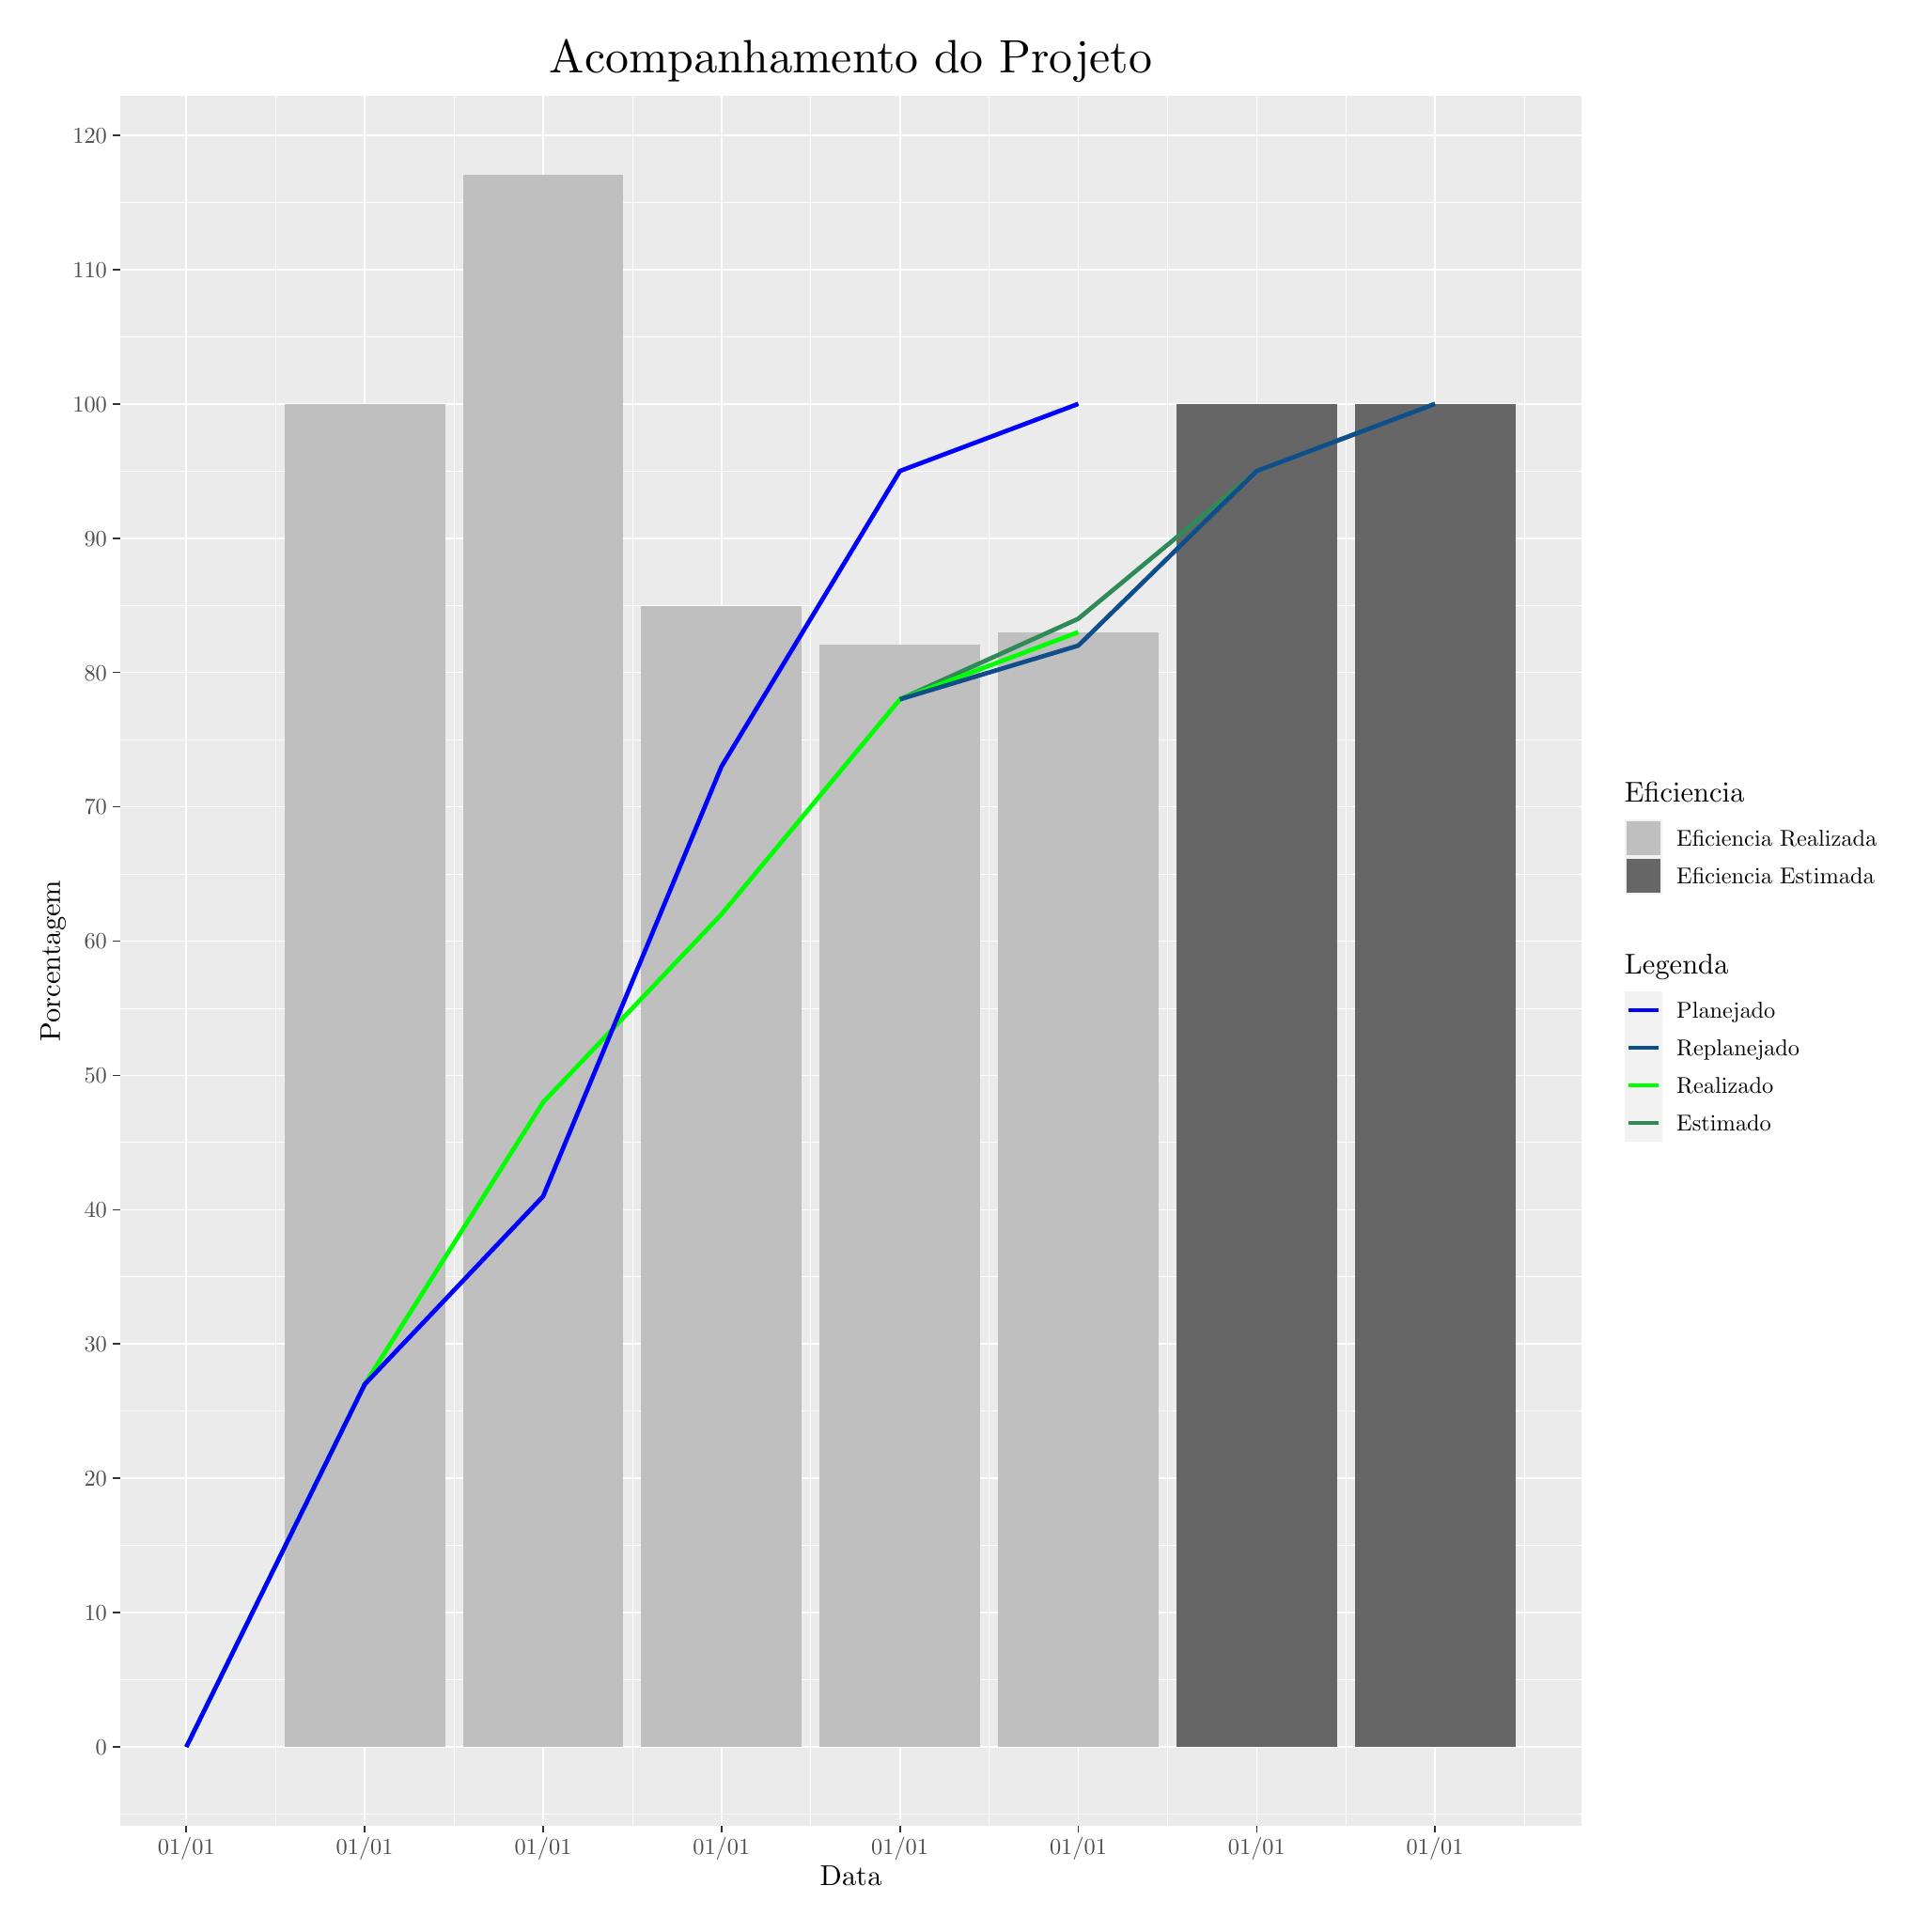
\begin{tikzpicture}[x=1pt,y=1pt]
\definecolor{fillColor}{RGB}{255,255,255}
\path[use as bounding box,fill=fillColor,fill opacity=0.00] (0,0) rectangle (722.70,722.70);
\begin{scope}
\path[clip] (  0.00,  0.00) rectangle (722.70,722.70);
\definecolor{drawColor}{RGB}{255,255,255}
\definecolor{fillColor}{RGB}{255,255,255}

\path[draw=drawColor,line width= 0.6pt,line join=round,line cap=round,fill=fillColor] (  0.00,  0.00) rectangle (722.70,722.70);
\end{scope}
\begin{scope}
\path[clip] ( 36.11, 30.69) rectangle (598.26,695.80);
\definecolor{fillColor}{gray}{0.92}

\path[fill=fillColor] ( 36.11, 30.69) rectangle (598.26,695.80);
\definecolor{drawColor}{RGB}{255,255,255}

\path[draw=drawColor,line width= 0.3pt,line join=round] ( 36.11, 35.09) --
	(598.26, 35.09);

\path[draw=drawColor,line width= 0.3pt,line join=round] ( 36.11, 86.74) --
	(598.26, 86.74);

\path[draw=drawColor,line width= 0.3pt,line join=round] ( 36.11,138.39) --
	(598.26,138.39);

\path[draw=drawColor,line width= 0.3pt,line join=round] ( 36.11,190.04) --
	(598.26,190.04);

\path[draw=drawColor,line width= 0.3pt,line join=round] ( 36.11,241.68) --
	(598.26,241.68);

\path[draw=drawColor,line width= 0.3pt,line join=round] ( 36.11,293.33) --
	(598.26,293.33);

\path[draw=drawColor,line width= 0.3pt,line join=round] ( 36.11,344.98) --
	(598.26,344.98);

\path[draw=drawColor,line width= 0.3pt,line join=round] ( 36.11,396.63) --
	(598.26,396.63);

\path[draw=drawColor,line width= 0.3pt,line join=round] ( 36.11,448.27) --
	(598.26,448.27);

\path[draw=drawColor,line width= 0.3pt,line join=round] ( 36.11,499.92) --
	(598.26,499.92);

\path[draw=drawColor,line width= 0.3pt,line join=round] ( 36.11,551.57) --
	(598.26,551.57);

\path[draw=drawColor,line width= 0.3pt,line join=round] ( 36.11,603.22) --
	(598.26,603.22);

\path[draw=drawColor,line width= 0.3pt,line join=round] ( 36.11,654.86) --
	(598.26,654.86);

\path[draw=drawColor,line width= 0.3pt,line join=round] ( 95.96, 30.69) --
	( 95.96,695.80);

\path[draw=drawColor,line width= 0.3pt,line join=round] (164.56, 30.69) --
	(164.56,695.80);

\path[draw=drawColor,line width= 0.3pt,line join=round] (233.16, 30.69) --
	(233.16,695.80);

\path[draw=drawColor,line width= 0.3pt,line join=round] (301.75, 30.69) --
	(301.75,695.80);

\path[draw=drawColor,line width= 0.3pt,line join=round] (370.35, 30.69) --
	(370.35,695.80);

\path[draw=drawColor,line width= 0.3pt,line join=round] (438.95, 30.69) --
	(438.95,695.80);

\path[draw=drawColor,line width= 0.3pt,line join=round] (507.54, 30.69) --
	(507.54,695.80);

\path[draw=drawColor,line width= 0.3pt,line join=round] (576.14, 30.69) --
	(576.14,695.80);

\path[draw=drawColor,line width= 0.6pt,line join=round] ( 36.11, 60.92) --
	(598.26, 60.92);

\path[draw=drawColor,line width= 0.6pt,line join=round] ( 36.11,112.57) --
	(598.26,112.57);

\path[draw=drawColor,line width= 0.6pt,line join=round] ( 36.11,164.21) --
	(598.26,164.21);

\path[draw=drawColor,line width= 0.6pt,line join=round] ( 36.11,215.86) --
	(598.26,215.86);

\path[draw=drawColor,line width= 0.6pt,line join=round] ( 36.11,267.51) --
	(598.26,267.51);

\path[draw=drawColor,line width= 0.6pt,line join=round] ( 36.11,319.16) --
	(598.26,319.16);

\path[draw=drawColor,line width= 0.6pt,line join=round] ( 36.11,370.80) --
	(598.26,370.80);

\path[draw=drawColor,line width= 0.6pt,line join=round] ( 36.11,422.45) --
	(598.26,422.45);

\path[draw=drawColor,line width= 0.6pt,line join=round] ( 36.11,474.10) --
	(598.26,474.10);

\path[draw=drawColor,line width= 0.6pt,line join=round] ( 36.11,525.75) --
	(598.26,525.75);

\path[draw=drawColor,line width= 0.6pt,line join=round] ( 36.11,577.39) --
	(598.26,577.39);

\path[draw=drawColor,line width= 0.6pt,line join=round] ( 36.11,629.04) --
	(598.26,629.04);

\path[draw=drawColor,line width= 0.6pt,line join=round] ( 36.11,680.69) --
	(598.26,680.69);

\path[draw=drawColor,line width= 0.6pt,line join=round] ( 61.66, 30.69) --
	( 61.66,695.80);

\path[draw=drawColor,line width= 0.6pt,line join=round] (130.26, 30.69) --
	(130.26,695.80);

\path[draw=drawColor,line width= 0.6pt,line join=round] (198.86, 30.69) --
	(198.86,695.80);

\path[draw=drawColor,line width= 0.6pt,line join=round] (267.45, 30.69) --
	(267.45,695.80);

\path[draw=drawColor,line width= 0.6pt,line join=round] (336.05, 30.69) --
	(336.05,695.80);

\path[draw=drawColor,line width= 0.6pt,line join=round] (404.65, 30.69) --
	(404.65,695.80);

\path[draw=drawColor,line width= 0.6pt,line join=round] (473.25, 30.69) --
	(473.25,695.80);

\path[draw=drawColor,line width= 0.6pt,line join=round] (541.84, 30.69) --
	(541.84,695.80);
\definecolor{fillColor}{gray}{0.75}

\path[fill=fillColor] ( 99.39, 60.92) rectangle (161.13,577.39);

\path[fill=fillColor] (167.99, 60.92) rectangle (229.73,665.57);

\path[fill=fillColor] (236.59, 60.92) rectangle (298.32,499.57);

\path[fill=fillColor] (305.18, 60.92) rectangle (366.92,484.97);

\path[fill=fillColor] (373.78, 60.92) rectangle (435.52,489.59);
\definecolor{fillColor}{gray}{0.40}

\path[fill=fillColor] (442.38, 60.92) rectangle (504.11,577.39);

\path[fill=fillColor] (510.97, 60.92) rectangle (572.71,577.39);
\definecolor{drawColor}{RGB}{46,139,87}

\path[draw=drawColor,line width= 1.7pt,line join=round] (336.05,463.77) --
	(404.65,494.76) --
	(473.25,551.57) --
	(541.84,577.39);
\definecolor{drawColor}{RGB}{0,255,0}

\path[draw=drawColor,line width= 1.7pt,line join=round] ( 61.66, 60.92) --
	(130.26,200.37) --
	(198.86,308.83) --
	(267.45,381.13) --
	(336.05,463.77) --
	(404.65,489.59);
\definecolor{drawColor}{RGB}{0,0,255}

\path[draw=drawColor,line width= 1.7pt,line join=round] ( 61.66, 60.92) --
	(130.26,200.37) --
	(198.86,272.67) --
	(267.45,437.94) --
	(336.05,551.57) --
	(404.65,577.39);
\definecolor{drawColor}{RGB}{16,78,139}

\path[draw=drawColor,line width= 1.7pt,line join=round] (336.05,463.77) --
	(404.65,484.43) --
	(473.25,551.57) --
	(541.84,577.39);
\end{scope}
\begin{scope}
\path[clip] (  0.00,  0.00) rectangle (722.70,722.70);
\definecolor{drawColor}{gray}{0.30}

\node[text=drawColor,anchor=base east,inner sep=0pt, outer sep=0pt, scale=  0.88] at ( 31.16, 57.89) {0};

\node[text=drawColor,anchor=base east,inner sep=0pt, outer sep=0pt, scale=  0.88] at ( 31.16,109.54) {10};

\node[text=drawColor,anchor=base east,inner sep=0pt, outer sep=0pt, scale=  0.88] at ( 31.16,161.18) {20};

\node[text=drawColor,anchor=base east,inner sep=0pt, outer sep=0pt, scale=  0.88] at ( 31.16,212.83) {30};

\node[text=drawColor,anchor=base east,inner sep=0pt, outer sep=0pt, scale=  0.88] at ( 31.16,264.48) {40};

\node[text=drawColor,anchor=base east,inner sep=0pt, outer sep=0pt, scale=  0.88] at ( 31.16,316.13) {50};

\node[text=drawColor,anchor=base east,inner sep=0pt, outer sep=0pt, scale=  0.88] at ( 31.16,367.77) {60};

\node[text=drawColor,anchor=base east,inner sep=0pt, outer sep=0pt, scale=  0.88] at ( 31.16,419.42) {70};

\node[text=drawColor,anchor=base east,inner sep=0pt, outer sep=0pt, scale=  0.88] at ( 31.16,471.07) {80};

\node[text=drawColor,anchor=base east,inner sep=0pt, outer sep=0pt, scale=  0.88] at ( 31.16,522.71) {90};

\node[text=drawColor,anchor=base east,inner sep=0pt, outer sep=0pt, scale=  0.88] at ( 31.16,574.36) {100};

\node[text=drawColor,anchor=base east,inner sep=0pt, outer sep=0pt, scale=  0.88] at ( 31.16,626.01) {110};

\node[text=drawColor,anchor=base east,inner sep=0pt, outer sep=0pt, scale=  0.88] at ( 31.16,677.66) {120};
\end{scope}
\begin{scope}
\path[clip] (  0.00,  0.00) rectangle (722.70,722.70);
\definecolor{drawColor}{gray}{0.20}

\path[draw=drawColor,line width= 0.6pt,line join=round] ( 33.36, 60.92) --
	( 36.11, 60.92);

\path[draw=drawColor,line width= 0.6pt,line join=round] ( 33.36,112.57) --
	( 36.11,112.57);

\path[draw=drawColor,line width= 0.6pt,line join=round] ( 33.36,164.21) --
	( 36.11,164.21);

\path[draw=drawColor,line width= 0.6pt,line join=round] ( 33.36,215.86) --
	( 36.11,215.86);

\path[draw=drawColor,line width= 0.6pt,line join=round] ( 33.36,267.51) --
	( 36.11,267.51);

\path[draw=drawColor,line width= 0.6pt,line join=round] ( 33.36,319.16) --
	( 36.11,319.16);

\path[draw=drawColor,line width= 0.6pt,line join=round] ( 33.36,370.80) --
	( 36.11,370.80);

\path[draw=drawColor,line width= 0.6pt,line join=round] ( 33.36,422.45) --
	( 36.11,422.45);

\path[draw=drawColor,line width= 0.6pt,line join=round] ( 33.36,474.10) --
	( 36.11,474.10);

\path[draw=drawColor,line width= 0.6pt,line join=round] ( 33.36,525.75) --
	( 36.11,525.75);

\path[draw=drawColor,line width= 0.6pt,line join=round] ( 33.36,577.39) --
	( 36.11,577.39);

\path[draw=drawColor,line width= 0.6pt,line join=round] ( 33.36,629.04) --
	( 36.11,629.04);

\path[draw=drawColor,line width= 0.6pt,line join=round] ( 33.36,680.69) --
	( 36.11,680.69);
\end{scope}
\begin{scope}
\path[clip] (  0.00,  0.00) rectangle (722.70,722.70);
\definecolor{drawColor}{gray}{0.20}

\path[draw=drawColor,line width= 0.6pt,line join=round] ( 61.66, 27.94) --
	( 61.66, 30.69);

\path[draw=drawColor,line width= 0.6pt,line join=round] (130.26, 27.94) --
	(130.26, 30.69);

\path[draw=drawColor,line width= 0.6pt,line join=round] (198.86, 27.94) --
	(198.86, 30.69);

\path[draw=drawColor,line width= 0.6pt,line join=round] (267.45, 27.94) --
	(267.45, 30.69);

\path[draw=drawColor,line width= 0.6pt,line join=round] (336.05, 27.94) --
	(336.05, 30.69);

\path[draw=drawColor,line width= 0.6pt,line join=round] (404.65, 27.94) --
	(404.65, 30.69);

\path[draw=drawColor,line width= 0.6pt,line join=round] (473.25, 27.94) --
	(473.25, 30.69);

\path[draw=drawColor,line width= 0.6pt,line join=round] (541.84, 27.94) --
	(541.84, 30.69);
\end{scope}
\begin{scope}
\path[clip] (  0.00,  0.00) rectangle (722.70,722.70);
\definecolor{drawColor}{gray}{0.30}

\node[text=drawColor,anchor=base,inner sep=0pt, outer sep=0pt, scale=  0.88] at ( 61.66, 19.68) {01/01};

\node[text=drawColor,anchor=base,inner sep=0pt, outer sep=0pt, scale=  0.88] at (130.26, 19.68) {01/01};

\node[text=drawColor,anchor=base,inner sep=0pt, outer sep=0pt, scale=  0.88] at (198.86, 19.68) {01/01};

\node[text=drawColor,anchor=base,inner sep=0pt, outer sep=0pt, scale=  0.88] at (267.45, 19.68) {01/01};

\node[text=drawColor,anchor=base,inner sep=0pt, outer sep=0pt, scale=  0.88] at (336.05, 19.68) {01/01};

\node[text=drawColor,anchor=base,inner sep=0pt, outer sep=0pt, scale=  0.88] at (404.65, 19.68) {01/01};

\node[text=drawColor,anchor=base,inner sep=0pt, outer sep=0pt, scale=  0.88] at (473.25, 19.68) {01/01};

\node[text=drawColor,anchor=base,inner sep=0pt, outer sep=0pt, scale=  0.88] at (541.84, 19.68) {01/01};
\end{scope}
\begin{scope}
\path[clip] (  0.00,  0.00) rectangle (722.70,722.70);
\definecolor{drawColor}{RGB}{0,0,0}

\node[text=drawColor,anchor=base,inner sep=0pt, outer sep=0pt, scale=  1.10] at (317.19,  7.64) {Data};
\end{scope}
\begin{scope}
\path[clip] (  0.00,  0.00) rectangle (722.70,722.70);
\definecolor{drawColor}{RGB}{0,0,0}

\node[text=drawColor,rotate= 90.00,anchor=base,inner sep=0pt, outer sep=0pt, scale=  1.10] at ( 13.08,363.24) {Porcentagem};
\end{scope}
\begin{scope}
\path[clip] (  0.00,  0.00) rectangle (722.70,722.70);
\definecolor{fillColor}{RGB}{255,255,255}

\path[fill=fillColor] (609.26,383.20) rectangle (717.20,438.32);
\end{scope}
\begin{scope}
\path[clip] (  0.00,  0.00) rectangle (722.70,722.70);
\definecolor{drawColor}{RGB}{0,0,0}

\node[text=drawColor,anchor=base west,inner sep=0pt, outer sep=0pt, scale=  1.10] at (614.76,424.18) {Eficiencia};
\end{scope}
\begin{scope}
\path[clip] (  0.00,  0.00) rectangle (722.70,722.70);
\definecolor{fillColor}{gray}{0.95}

\path[fill=fillColor] (614.76,403.15) rectangle (629.22,417.61);
\end{scope}
\begin{scope}
\path[clip] (  0.00,  0.00) rectangle (722.70,722.70);
\definecolor{fillColor}{gray}{0.75}

\path[fill=fillColor] (615.48,403.86) rectangle (628.51,416.90);
\end{scope}
\begin{scope}
\path[clip] (  0.00,  0.00) rectangle (722.70,722.70);
\definecolor{fillColor}{gray}{0.75}

\path[fill=fillColor] (615.48,403.86) rectangle (628.51,416.90);
\end{scope}
\begin{scope}
\path[clip] (  0.00,  0.00) rectangle (722.70,722.70);
\definecolor{fillColor}{gray}{0.95}

\path[fill=fillColor] (614.76,388.70) rectangle (629.22,403.15);
\end{scope}
\begin{scope}
\path[clip] (  0.00,  0.00) rectangle (722.70,722.70);
\definecolor{fillColor}{gray}{0.40}

\path[fill=fillColor] (615.48,389.41) rectangle (628.51,402.44);
\end{scope}
\begin{scope}
\path[clip] (  0.00,  0.00) rectangle (722.70,722.70);
\definecolor{fillColor}{gray}{0.40}

\path[fill=fillColor] (615.48,389.41) rectangle (628.51,402.44);
\end{scope}
\begin{scope}
\path[clip] (  0.00,  0.00) rectangle (722.70,722.70);
\definecolor{drawColor}{RGB}{0,0,0}

\node[text=drawColor,anchor=base west,inner sep=0pt, outer sep=0pt, scale=  0.88] at (634.72,407.35) {Eficiencia Realizada};
\end{scope}
\begin{scope}
\path[clip] (  0.00,  0.00) rectangle (722.70,722.70);
\definecolor{drawColor}{RGB}{0,0,0}

\node[text=drawColor,anchor=base west,inner sep=0pt, outer sep=0pt, scale=  0.88] at (634.72,392.90) {Eficiencia Estimada};
\end{scope}
\begin{scope}
\path[clip] (  0.00,  0.00) rectangle (722.70,722.70);
\definecolor{fillColor}{RGB}{255,255,255}

\path[fill=fillColor] (609.26,288.17) rectangle (687.51,372.20);
\end{scope}
\begin{scope}
\path[clip] (  0.00,  0.00) rectangle (722.70,722.70);
\definecolor{drawColor}{RGB}{0,0,0}

\node[text=drawColor,anchor=base west,inner sep=0pt, outer sep=0pt, scale=  1.10] at (614.76,358.05) {Legenda};
\end{scope}
\begin{scope}
\path[clip] (  0.00,  0.00) rectangle (722.70,722.70);
\definecolor{fillColor}{gray}{0.95}

\path[fill=fillColor] (614.76,337.03) rectangle (629.22,351.48);
\end{scope}
\begin{scope}
\path[clip] (  0.00,  0.00) rectangle (722.70,722.70);
\definecolor{drawColor}{RGB}{0,0,255}

\path[draw=drawColor,line width= 1.7pt,line join=round] (616.21,344.26) -- (627.77,344.26);
\end{scope}
\begin{scope}
\path[clip] (  0.00,  0.00) rectangle (722.70,722.70);
\definecolor{drawColor}{RGB}{0,0,255}

\path[draw=drawColor,line width= 1.7pt,line join=round] (616.21,344.26) -- (627.77,344.26);
\end{scope}
\begin{scope}
\path[clip] (  0.00,  0.00) rectangle (722.70,722.70);
\definecolor{drawColor}{RGB}{0,0,255}

\path[draw=drawColor,line width= 1.7pt,line join=round] (616.21,344.26) -- (627.77,344.26);
\end{scope}
\begin{scope}
\path[clip] (  0.00,  0.00) rectangle (722.70,722.70);
\definecolor{drawColor}{RGB}{0,0,255}

\path[draw=drawColor,line width= 1.7pt,line join=round] (616.21,344.26) -- (627.77,344.26);
\end{scope}
\begin{scope}
\path[clip] (  0.00,  0.00) rectangle (722.70,722.70);
\definecolor{fillColor}{gray}{0.95}

\path[fill=fillColor] (614.76,322.58) rectangle (629.22,337.03);
\end{scope}
\begin{scope}
\path[clip] (  0.00,  0.00) rectangle (722.70,722.70);
\definecolor{drawColor}{RGB}{16,78,139}

\path[draw=drawColor,line width= 1.7pt,line join=round] (616.21,329.80) -- (627.77,329.80);
\end{scope}
\begin{scope}
\path[clip] (  0.00,  0.00) rectangle (722.70,722.70);
\definecolor{drawColor}{RGB}{16,78,139}

\path[draw=drawColor,line width= 1.7pt,line join=round] (616.21,329.80) -- (627.77,329.80);
\end{scope}
\begin{scope}
\path[clip] (  0.00,  0.00) rectangle (722.70,722.70);
\definecolor{drawColor}{RGB}{16,78,139}

\path[draw=drawColor,line width= 1.7pt,line join=round] (616.21,329.80) -- (627.77,329.80);
\end{scope}
\begin{scope}
\path[clip] (  0.00,  0.00) rectangle (722.70,722.70);
\definecolor{drawColor}{RGB}{16,78,139}

\path[draw=drawColor,line width= 1.7pt,line join=round] (616.21,329.80) -- (627.77,329.80);
\end{scope}
\begin{scope}
\path[clip] (  0.00,  0.00) rectangle (722.70,722.70);
\definecolor{fillColor}{gray}{0.95}

\path[fill=fillColor] (614.76,308.12) rectangle (629.22,322.58);
\end{scope}
\begin{scope}
\path[clip] (  0.00,  0.00) rectangle (722.70,722.70);
\definecolor{drawColor}{RGB}{0,255,0}

\path[draw=drawColor,line width= 1.7pt,line join=round] (616.21,315.35) -- (627.77,315.35);
\end{scope}
\begin{scope}
\path[clip] (  0.00,  0.00) rectangle (722.70,722.70);
\definecolor{drawColor}{RGB}{0,255,0}

\path[draw=drawColor,line width= 1.7pt,line join=round] (616.21,315.35) -- (627.77,315.35);
\end{scope}
\begin{scope}
\path[clip] (  0.00,  0.00) rectangle (722.70,722.70);
\definecolor{drawColor}{RGB}{0,255,0}

\path[draw=drawColor,line width= 1.7pt,line join=round] (616.21,315.35) -- (627.77,315.35);
\end{scope}
\begin{scope}
\path[clip] (  0.00,  0.00) rectangle (722.70,722.70);
\definecolor{drawColor}{RGB}{0,255,0}

\path[draw=drawColor,line width= 1.7pt,line join=round] (616.21,315.35) -- (627.77,315.35);
\end{scope}
\begin{scope}
\path[clip] (  0.00,  0.00) rectangle (722.70,722.70);
\definecolor{fillColor}{gray}{0.95}

\path[fill=fillColor] (614.76,293.67) rectangle (629.22,308.12);
\end{scope}
\begin{scope}
\path[clip] (  0.00,  0.00) rectangle (722.70,722.70);
\definecolor{drawColor}{RGB}{46,139,87}

\path[draw=drawColor,line width= 1.7pt,line join=round] (616.21,300.90) -- (627.77,300.90);
\end{scope}
\begin{scope}
\path[clip] (  0.00,  0.00) rectangle (722.70,722.70);
\definecolor{drawColor}{RGB}{46,139,87}

\path[draw=drawColor,line width= 1.7pt,line join=round] (616.21,300.90) -- (627.77,300.90);
\end{scope}
\begin{scope}
\path[clip] (  0.00,  0.00) rectangle (722.70,722.70);
\definecolor{drawColor}{RGB}{46,139,87}

\path[draw=drawColor,line width= 1.7pt,line join=round] (616.21,300.90) -- (627.77,300.90);
\end{scope}
\begin{scope}
\path[clip] (  0.00,  0.00) rectangle (722.70,722.70);
\definecolor{drawColor}{RGB}{46,139,87}

\path[draw=drawColor,line width= 1.7pt,line join=round] (616.21,300.90) -- (627.77,300.90);
\end{scope}
\begin{scope}
\path[clip] (  0.00,  0.00) rectangle (722.70,722.70);
\definecolor{drawColor}{RGB}{0,0,0}

\node[text=drawColor,anchor=base west,inner sep=0pt, outer sep=0pt, scale=  0.88] at (634.72,341.23) {Planejado};
\end{scope}
\begin{scope}
\path[clip] (  0.00,  0.00) rectangle (722.70,722.70);
\definecolor{drawColor}{RGB}{0,0,0}

\node[text=drawColor,anchor=base west,inner sep=0pt, outer sep=0pt, scale=  0.88] at (634.72,326.77) {Replanejado};
\end{scope}
\begin{scope}
\path[clip] (  0.00,  0.00) rectangle (722.70,722.70);
\definecolor{drawColor}{RGB}{0,0,0}

\node[text=drawColor,anchor=base west,inner sep=0pt, outer sep=0pt, scale=  0.88] at (634.72,312.32) {Realizado};
\end{scope}
\begin{scope}
\path[clip] (  0.00,  0.00) rectangle (722.70,722.70);
\definecolor{drawColor}{RGB}{0,0,0}

\node[text=drawColor,anchor=base west,inner sep=0pt, outer sep=0pt, scale=  0.88] at (634.72,297.87) {Estimado};
\end{scope}
\begin{scope}
\path[clip] (  0.00,  0.00) rectangle (722.70,722.70);
\definecolor{drawColor}{RGB}{0,0,0}

\node[text=drawColor,anchor=base,inner sep=0pt, outer sep=0pt, scale=  1.80] at (317.19,704.80) {Acompanhamento do Projeto};
\end{scope}
\end{tikzpicture}
